\documentclass{beamer}

\usepackage{graphicx}


\usetheme{Madrid}

\DeclareMathOperator{\RSS}{RSS}
\DeclareMathOperator*{\Argmin}{argmin}
\DeclareMathOperator*{\Argmax}{argmax}

\newcommand{\RR}{\mathbb{R}}
\newcommand{\va}{\boldsymbol{a}}
\newcommand{\vb}{\boldsymbol{b}}
\newcommand{\vx}{\boldsymbol{x}}
\newcommand{\vy}{\boldsymbol{y}}
\newcommand{\vz}{\boldsymbol{z}}
\newcommand{\vW}{\boldsymbol{W}}
\newcommand{\lra}{\longrightarrow}

\begin{document}
    
\setlength{\parskip}{1em}
\begin{frame}
    \title{Introduction to Neural Networks}
    \date{DATA 607 --- Session 8 --- 22.03.2020}
    \maketitle
\end{frame}

\begin{frame}{What is a neural network?}
    A neural network consists of \textbf{neurons} or \textbf{units}.
    Neurons have \textbf{inputs}, \textbf{outputs}, and \textbf{activations}.
    Connections between these neurons have \textbf{weights}.
    Neurons are organized into \textbf{layers}. \textbf{Hidden layers}
    are sandwiched between an \textbf{input layer} and an \textbf{output layer}.

    Linear regression, logistic regression, and perceptron classification are all
    neural networks, degenerate in the sense that they have no hidden layers.
\end{frame}

\begin{frame}{}
    More formally, a neural network is a function
    \[
        N:\RR^p\lra \RR^q
    \]
    constructed in a particular way.

    \begin{center}
    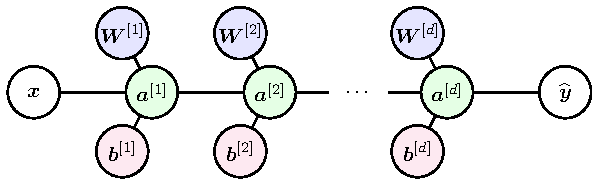
\includegraphics{basic_nn_vectorized.pdf}
    \end{center}
\end{frame}

\begin{frame}{}
    \begin{align*}
        \text{depth of network (number of layers):\quad}&d\\
        \text{number of neurons in layer $\ell$:\quad}&p_\ell\\
        \text{activation (output) of neuron $k$ in layer $\ell$:\quad}
        & a_k^{[\ell]}\\[1ex]
        \text{bias of neuron $k$ in layer $\ell$:\quad}& b_k^{[\ell]}\\[1ex]
        \text{\parbox{3in}{\raggedleft weight of the connection between neuron $j$\\
        in layer $\ell$ and neuron $i$ in layer $\ell+1$:}\quad}& w^{[\ell]}_{ij}\\
        \text{activation function in layer $\ell$:\quad}&h
    \end{align*}

    \[
        a^{[\ell+1]}_i = h\left(z_i^{[\ell+1]}\right),
        \quad\text{where}\quad
        z_i^{[\ell+1]}=b_i^{[\ell]} + \sum_{j=1}^{p_\ell} w_{ij}^{[\ell]}a_j^{[\ell]}
    \]
\end{frame}

\begin{frame}{}
    Vectorize:
    \[
        \vz^{[\ell]} = \begin{bmatrix}
            z^{[\ell]}_1\\\vdots\\z^{[\ell]}_{p_\ell}
        \end{bmatrix}\in\RR^{p_\ell},\quad
        \va^{[\ell]} = \begin{bmatrix}
            a^{[\ell]}_1\\\vdots\\a^{[\ell]}_{p_\ell}
        \end{bmatrix}\in\RR^{p_\ell},
    \]
    \[
        \vb^{[\ell]} = \begin{bmatrix}
            b^{[\ell]}_1\\\vdots\\b^{[\ell]}_{p_\ell}
        \end{bmatrix}\in\RR^{p_\ell},\quad
        \vW^{[\ell]} = \begin{bmatrix}
            w^{[\ell]}_{11}&\cdots &w^{[\ell]}_{1p_\ell}\\
            \vdots & \ddots & \vdots\\
            w^{[\ell]}_{p_{\ell+1}1}&\cdots &w^{[\ell]}_{1p_\ell}
        \end{bmatrix}\in\RR^{p_{\ell+1}\times p_\ell}
    \]

    Apply $h$ componentwise:
    \[
        \va_i^{[\ell + 1]} = h\left(\vz^{[\ell+1]}\right)=
        h\left(\vb^{[\ell]} + \vW^{[\ell]}\va^{[\ell]}\right)
    \]

    Useful intermediate quantity:
    \[
        \vb^{[\ell]} + \vW^{[\ell]}\va^{[\ell]}
    \]
\end{frame}

\begin{frame}{}
    The process of computing $\hat{\vy}$ from $\vx$,
    given $\vb^{[\ell]}$ and $\vW^{[\ell]}$, $\ell=1,\ldots,d$,
    is called \textbf{forward propagation} of data.

    A \textbf{loss function}, $L(\hat y, y)$,
    asseses a penalty based on the error in approximating $\vy$ by $\hat\vy$.

    The total loss associated to a training set
    \[
        T=\{(\vx_1,\vy_1),\ldots,(\vx_n, \vy_n)\}
    \]
    is called the \textbf{cost} of $T$:
    \[
        C(T) = \sum_{i=1}^n L(\hat \vy_i, \vy_i)
    \]
    We adjust the variables $\vb^{[\ell]}$ and $\vW^{[\ell]}$ based on
    the derivatives
    \[
        \frac{\partial C}{\partial b^{[\ell]}_i}
        \quad\text{and}\quad
        \frac{\partial C}{\partial w^{[\ell]}_{ij}}
    \]
\end{frame}
\end{document}